\documentclass[conference]{IEEEtran}
\IEEEoverridecommandlockouts
% The preceding line is only needed to identify funding in the first footnote. If that is unneeded, please comment it out.
\usepackage{cite}
\usepackage{amsmath,amssymb,amsfonts}
\usepackage{algorithmic}
\usepackage{graphicx}
\usepackage{appendix}
\usepackage{textcomp}
\usepackage{xcolor}
\usepackage{multicol}
\usepackage{tabularx}
\usepackage{relsize}
\usepackage{float}
\def\BibTeX{{\rm B\kern-.05em{\sc i\kern-.025em b}\kern-.08em
    T\kern-.1667em\lower.7ex\hbox{E}\kern-.125emX}}
\begin{document}

\title{FedMix and FedAdp\\
}

\author{\IEEEauthorblockN{1\textsuperscript{st} Luca Marcellino}
\IEEEauthorblockA{\textit{Politecnico di Torino}\\
Turin, Italy \\
s292950@studenti.polito.it}
\and
\IEEEauthorblockN{2\textsuperscript{nd} Luca Villani}
\IEEEauthorblockA{\textit{Politecnico di Torino}\\
Turin, Italy \\
s304992@studenti.polito.it}
\and
\IEEEauthorblockN{3\textsuperscript{rd} Edoardo Bonelli}
\IEEEauthorblockA{\textit{Politecnico di Torino}\\
Turin, Italy \\
s306073@studenti.polito.it}
}

\maketitle
\thispagestyle{plain}
\pagestyle{plain}


\begin{abstract}
In this work we tried two possible new scenarios related to the Federated Learning setting. Indeed we studied a new approach to compute normalization, based on a linear combination of the normalization weight from the Batch Norm and the Group Norm, we have tried it in different models. Then we tried, also, to figure out a framework in which is possible adjust the memory that we want to allocate to the training phase based on the device on which the model is executed. Moreover in this case is also possible to leave the choice to the user on how much memory he wants to allocate for this kind of task. We called this two methods Federated Mix (\textbf{FedMix}), since we mix two kinds of normalization, and Federate Adaptive (\textbf{FedAdp}), since we will have different batch sizes (user based) and the normalization layers will adapt based on the latter.
\end{abstract}


\section{Introduction}
In recent years, the idea of processing data but also keeping the idea of privacy in mind is gaining ground. All this can be summarised in the idea of \textbf{Federated Learning}. This concept was born in 2016 through a Google search.

Federated learning is a method of training machine learning models on large amounts of data without collecting and storing the data on a central server. It involves sending a model to multiple devices, where the devices train the model on their local data and send the updated model back to a central server. The server then aggregates the models from all the devices to create a global model. This process is repeated until the global model is sufficiently accurate. 

Federated learning allows organizations to train models on sensitive data without compromising the privacy of individuals, and it allows organizations to train models on a larger and more diverse dataset than would be possible with a single device or server. Federated learning has the potential to revolutionize the way organizations approach data processing and machine learning\cite{b1}.

In this scenario, we decided to try out two different implementations. One of them is at the level of the ResNet50 structure, in fact we decided to perform a linear combination of the Batch and Group norm. In the second, we decided to allocate different sizes of memory to the clients, and see which normalisation worked best.

We tested our code in the area of image recognition divided into 10 classes (CIFAR10). In addition, both IID and Non-IID balanced/unbalanced settings were tested.

\section{Related Work}

Several approaches related to Federated Learning have emerged in recent years. Our experiments were based on the combination of two normalisations. The first Batch Norm \cite{b2} is best in the case of IID settings or when we have high batch sizes. Since as soon as we deviate from the conditions mentioned above, we no longer have the desired results, we decided to also try the Gruop Norm \cite{b3}. The latter turned out to have better effects in the case of Non-IID and smaller batch sizes.

With regard to the methods used in Federated Learning, various approaches famous in the literature and implementations were used to test our new normalisation method. The first one tested was the Federated Average (FedAvg) \cite{b4} in which weights are averaged for server uploads. Subsequently, the Federated Group Knowledge Transfer (FedGKT)\cite{b5}  was also tested, which is a process by which knowledge and expertise is shared and exchanged between different groups or organisations within a larger federation or network.

As an architecture, instead, a ResNet50 \cite{b6} was used with a few modifications related to the type of method used for uploading to the central server. In fact, in the case of FedGKT, the architectures used were ResNet8 for the client and ResNet49 for the server. 

Finally, a network attack test was also carried out in which a Gradient Inverse Attack \cite{b7} was tested. With this approach, one tries, through weights, to derive the initial image and thus violate privacy.

\subsection{Database}
To test the algorithms we used CIFAR-10 that is a dataset of 60,000 32x32 color images in 10 classes, with 6,000 images per class. The classes are airplane, automobile, bird, cat, deer, dog, frog, horse, ship, and truck. It is commonly used as a benchmark for image classification and computer vision models. CIFAR-10 was developed by the Canadian Institute for Advanced Research (CIFAR) and is widely used in research and education.

\section{Methods}

Before illustrating our proposed methods, it is necessary to make a brief introduction and explanation of the standards used in the Federated Mix and in which applications they are used.

\subsection{Batch Normalization}

Batch normalization is a technique used to improve the performance and stability of deep learning models, which are neural networks with many layers. It works by normalizing the activations of the layers in the network, which can help to reduce overfitting and improve the generalization of the model to new data.

One advantage of using batch normalization in image recognition models is that it can significantly improve the training speed and convergence of the model. It can also help to reduce the sensitivity of the model to the initial values of the weights and biases, which can improve the stability of the model. Additionally, it can help to reduce overfitting by adding some noise to the activations, which can make the model more robust to small perturbations in the input data.

However, it is important to note that batch normalization requires a sufficient batch size in order to accurately estimate the mean and standard deviation, and it may not be effective in some cases if the batch size is too small.

Let us use B to denote a mini-batch of size m of the entire training set. The empirical mean and variance of B could thus be denoted as \cite{b8}:

\begin{multicols}{2}
  \begin{equation}
    \mu _{B}={\frac {1}{m}}\sum _{i=1}^{m}x_{i}
  \end{equation}\break
  \begin{equation}
    \sigma _{B}^{2}={\frac {1}{m}}\sum _{i=1}^{m}(x_{i}-\mu _{B})^{2}
  \end{equation}
\end{multicols}

For a layer of the network with d-dimensional input, $x = (x^{(1)},...,x^{(d)})$ , each dimension of its input is then normalized (i.e. re-centered and re-scaled) separately. 
\begin{equation}
 {\hat {x}}_{i}^{(k)}={\frac {x_{i}^{(k)}-\mu _{B}^{(k)}}{\sqrt {\left(\sigma _{B}^{(k)}\right)^{2}+\epsilon }}}
\end{equation}
Where $k \in [1,d]$.

\subsection{Group Normalization}

Group normalization is a variant of batch normalization, which is a technique used to improve the performance and stability of deep learning models.Also group normalization is used to normalize the activations of the layers in a neural network, which can help to reduce overfitting and improve the generalization of the model to new data. 

Again, the basic idea is to subtract the mean and divide by the standard deviation. This time, however, the normalisation takes place on channel groups instead of bacth size. So GN computations is independent of batch sizes, and its accuracy is stable in a wide range of batch sizes.

One advantage of group normalization compared to batch normalization is that it can be more computationally efficient, since it does not require the use of mini-batches. Moreover BN’s error increases rapidly when the batch size becomes smaller, caused by inaccurate batch statistics estimation. However, it may not be as effective as batch normalization in some cases, especially when the groups are too small or the data is highly correlated.

\subsection{\textbf{Federated Mix}}

The Federated Mix stems from the idea of the limitations mentioned above. In fact, as mentioned above, Batch normalisation does not have accurate results if the number of batches goes down but at the same time at high batches it achieves higher levels of accuracy. 

In addition, we realised that the performance of the two methods changed depending on the distribution of the data. In fact, Group normalisation performed better if the dataset was Non-IID unbalanced. In contrast, Batch normalisation worked better in the case of an IID, and therefore, balanced dataset.

Based on these assumptions, we decided to try to implement a neural network that could encapsulate both normalisation and take advantage of them. To do this, we decided to perform a linear combination of the two normalisation through two coefficients alpha\_b ($\alpha_b$) and alpha\_g ($\alpha_g$). 

\begin{equation}
    x = \alpha_b \cdot~ BN(x) + \alpha_g \cdot~ GN(x)
\end{equation}

Subsequently, we looked for which values of $\alpha_b$ and $\alpha_g$ maximised accuracy.

\subsection{\textbf{Federated Adaptive}}

Federated Adaptive (FedAdp) stems from the very idea of Federated Learning. In fact, the idea of this method is to focus on the memory used by the client in its model training process. In the more specific case of all clients, they can either choose the memory to be dedicated to training, or the device itself can communicate the memory it can dedicate based on the user's use of the device. 

We have called this method "Adaptive" because according to the memory dedicated by the device, and thus, the number of images per batch, the model decides whether to perform Batch or Group normalisation. In order to do this, we have, for the clients, a ResNet implemented as in the case of FedMix, in which the two coefficients will be set to 0 depending on which normalisation we want to use.

If from the client's point of view everything seems to be simple enough, the problems come from the server side. In fact, in this case we decided to test our idea by following the FedAvg model and then use the average of the weights. At this point, however, we decided to also use the FedMix model for the server and went looking for $\alpha_b$ and $\alpha_g$ parameters that would improve accuracy.
\section{Results}
\subsection{Centralized Experiment}
The performance of any model trained in a federated fashion is upper bounded by the results obtained in the centralized setting, i.e. the standard one. We therefore decided to test the ResNet-50 and the model itself as the first things on the centralised. We also decided to tune the parameters within these experiments. The tuned parameters were: learning rate, momentum and optimizer. As far as the weight decay is concerned, we fixed it at 0 due to computational power, but we have seen, also through other experiments in the papers, that it is the best choice.

In the table here, there are the results we decided to take into account. We decided not to use Adam as an optimizer for two main reasons: the first is that in the case of group norm SGD gives better results (Table \ref{tab:1} in the appendix), second because it needs a larger memory and our resources are limited. It might however be a good experiment to test the results also with Adam as an optimizer.
\begin{table}[H]
\begin{tabular}{|p{0.15\columnwidth}|p{0.15\columnwidth}|p{0.15\columnwidth}|p{0.15\columnwidth}|p{0.15\columnwidth}|}
\hline
{\textbf{\begin{tabular}[c]{@{}c@{}c@{}}\centerline{Norm}\end{tabular}}} 
& {\textbf{\begin{tabular}[c]{@{}c@{}c@{}}Learning \\ rate\end{tabular}}}
& {\textbf{\begin{tabular}[c]{@{}c@{}}\centerline{Momentum} \\\end{tabular}}}
& {\textbf{\begin{tabular}[c]{@{}c@{}c@{}}\centerline{Optimizer}\end{tabular}}}
& {\textbf{\begin{tabular}[c]{@{}c@{}c@{}}Test \\ Accuracy \\(\%)\end{tabular}}}\\ \hline

\rule[-4mm]{0mm}{1cm} {BN} & \centerline{0.1} & \centerline{0.5} & \centerline{SGD} & \centerline{81.0}\\\hline
\rule[-4mm]{0mm}{1cm} {\textbf{BN}} & \centerline{\textbf{0.1}} & \centerline{\textbf{0.9}} & \centerline{\textbf{SGD}} & \centerline{\textbf{85.0}}\\\hline
\rule[-4mm]{0mm}{1cm} {GN} & \centerline{0.1} & \centerline{0.5} & \centerline{SGD} & \centerline{81.0}\\\hline
\rule[-4mm]{0mm}{1cm} {\textbf{GN}} & \centerline{\textbf{0.1}} & \centerline{\textbf{0.9}} & \centerline{\textbf{SGD}} & \centerline{\textbf{83.0}}\\\hline
\end{tabular}
\end{table}
From the table, it is easy to see which results are best when the parameters vary. Nevertheless, we decided to test the implementations also on the FedAvg as a baseline to see which combination was best.

\subsection{Federated baseline Experiments}
As mentioned earlier, we decided to test the two implementations on FedAvg as well. To do this we decided to fix the normalization (we used batch) and decided to test with data distributed in IID and Non-IID.
\begin{table}[H]
\begin{tabular}{|p{0.15\columnwidth}|p{0.15\columnwidth}|p{0.15\columnwidth}|p{0.15\columnwidth}|p{0.15\columnwidth}|}
\hline
{\textbf{\begin{tabular}[c]{@{}c@{}c@{}}Distribution \\ data\end{tabular}}} 
& {\textbf{\begin{tabular}[c]{@{}c@{}c@{}}Learning \\ rate\end{tabular}}}
& {\textbf{\begin{tabular}[c]{@{}c@{}}\centerline{Momentum} \\\end{tabular}}}
& {\textbf{\begin{tabular}[c]{@{}c@{}c@{}}\centerline{Optimizer}\end{tabular}}}
& {\textbf{\begin{tabular}[c]{@{}c@{}c@{}}Test \\ Accuracy \\(\%)\end{tabular}}}\\ \hline

\rule[-4mm]{0mm}{1cm} {\textbf{IID}} & \centerline{\textbf{0.1}} & \centerline{\textbf{0.5}} & \centerline{\textbf{SGD}} & \centerline{\textbf{61.51}}\\\hline
\rule[-4mm]{0mm}{1cm} {IID} & \centerline{0.1} & \centerline{0.9} & \centerline{SGD} & \centerline{55.81}\\\hline
\rule[-4mm]{0mm}{1cm} {\textbf{Non-IID}} & \centerline{\textbf{0.1}} & \centerline{\textbf{0.5}} & \centerline{\textbf{SGD}} & \centerline{\textbf{18.56}}\\\hline
\rule[-4mm]{0mm}{1cm} {Non-IID} & \centerline{0.1} & \centerline{0.9} & \centerline{SGD} & \centerline{17.1}\\\hline
\end{tabular}
\end{table}
Looking at the results, one can immediately see how the trends are completely reversed. This is because it is not mandatory that the parameters that work best in centralized also work best in FedAvg. Given these results, we decided to run each of our experiments with momentum equal to 0.5, learning rate equal to 0.1 and SGD as the optimizer.

\subsection{Experiment Settings}
To carry out the experiments, we used the Kaggle GPU P100. Each method was tested in several possible scenarios.

In the FedAvg part, 50 total epochs and 5 local epochs were tested, the local batch size was set at 16. For this method, both the ResNet 50 with batch and group normalisation and the ResNet 50 with the linear combination of normalisations (FedMix) were tested.

For the FedGKT, on the other hand, 50 communications rounds were carried out with 10 local epochs, server side, and 1 epoch, client side. The local batch size was tested at both 128 and 16. Again, this was tested with both the ResNet 50 and the setting in FedMix.

Finally, we also tested the new FedAdp method. In this case, the weight update method is still a FedAvg. Again, this was tested for 50 total epochs and 5 local epochs. As far as the batch size is concerned, more information will be given in the subsection with the results.

\subsection{Gradient Inverse Attack Experiments}
To test privacy we decided to try an attack on our own network. To do this, we used a pretrained ResNet-50, on ImageNet, so that we could test whether this neural network could accurately defend privacy. We then performed a gradient inverse attack by verifying it on a FedAvg type algorithm.
Logically, to the attack was given the correct parameters of our model and was tested for 8000 iterations. In order to verify what has just been said, we decided to test it on three photos belonging to different classes: frog, boat and truck. 
\begin{figure}[H]
    \centering
    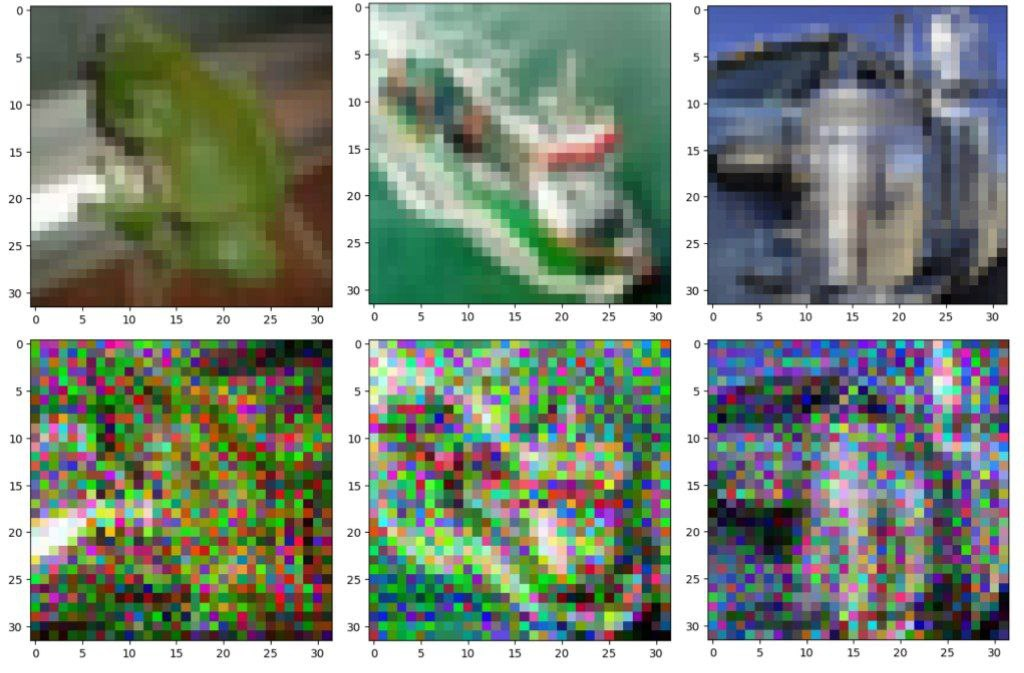
\includegraphics[width=\columnwidth]{Images/Comparison inverse attack.jpg}
    \caption{Original and reconstruct figures}
    \label{fig:1}
\end{figure}
Looking at the origin and reconstructed images, similarities can be seen, but they are still really difficult to recognize, so we believe that ResNet-50 is a fairly safe neural network.

\subsection{FedMix Experiments}
To carry out these experiments, we decided to set the local batch size equal to 16.

The first test performed is the comparison between FedMix and FedAvg in IID settings. 
\begin{table}[H]
\begin{tabular}{|p{0.12\columnwidth}|p{0.12\columnwidth}|p{0.12\columnwidth}|p{0.12\columnwidth}|p{0.12\columnwidth}|p{0.12\columnwidth}|}
\hline
& {\textbf{\begin{tabular}[c]{@{}c@{}c@{}}FedAvg \\ GN\end{tabular}}} 
& {\textbf{\begin{tabular}[c]{@{}c@{}c@{}}FedAvg \\ BN\end{tabular}}}
& {\textbf{\begin{tabular}[c]{@{}c@{}c@{}}FedMix\\ $\alpha_b$=0.5 \\ $\alpha_g$=0.5\end{tabular}}}
& {\textbf{\begin{tabular}[c]{@{}c@{}c@{}}FedMix\\ $\alpha_b$=0.9 \\ $\alpha_g$=0.1\end{tabular}}} 
& {\textbf{\begin{tabular}[c]{@{}c@{}c@{}}FedMix\\ $\alpha_b$=0.1\\ $\alpha_g$=0.9\end{tabular}}} \\ \hline

{\textbf{\begin{tabular}[c]{@{}c@{}c@{}}Test \\ Accuracy \\(\%)\end{tabular}}} & \rule[-4mm]{0mm}{1cm} {42.86} & \centerline{\textbf{61.51}} & \centerline{56.04} & \centerline{37.53} & \centerline{53.67}\\\hline
\end{tabular}
\end{table}
In this case, our method does not show any improvement, in fact it performs worse. However, a look at the graph Fig.\ref{fig:appendix1} (in the appendix) shows that our method performs better at low epochs.

As a second test, we tested our method in \textbf{Non-IID balanced} settings. The results obtained are as follows.
\begin{table}[H]
\begin{tabular}{|p{0.12\columnwidth}|p{0.12\columnwidth}|p{0.12\columnwidth}|p{0.12\columnwidth}|p{0.12\columnwidth}|p{0.12\columnwidth}|}
\hline
& {\textbf{\begin{tabular}[c]{@{}c@{}c@{}}FedAvg \\ GN\end{tabular}}} 
& {\textbf{\begin{tabular}[c]{@{}c@{}c@{}}FedAvg \\ BN\end{tabular}}}
& {\textbf{\begin{tabular}[c]{@{}c@{}c@{}}FedMix\\ $\alpha_b$=0.5 \\ $\alpha_g$=0.5\end{tabular}}}
& {\textbf{\begin{tabular}[c]{@{}c@{}c@{}}FedMix\\ $\alpha_b$=0.9 \\ $\alpha_g$=0.1\end{tabular}}} 
& {\textbf{\begin{tabular}[c]{@{}c@{}c@{}}FedMix\\ $\alpha_b$=0.1\\ $\alpha_g$=0.9\end{tabular}}} \\ \hline

{\textbf{\begin{tabular}[c]{@{}c@{}c@{}}Test \\ Accuracy \\(\%)\end{tabular}}} & \rule[-4mm]{0mm}{1cm} {19.52} & \centerline{18.56} & \centerline{20.57} & \centerline{12.91} & \centerline{\textbf{25.99}}\\\hline
\end{tabular}
\end{table}

In this case, it can be seen that our proposed method is far better. In fact, the delta between the methods is very high and at the $50^{th}$ epoch is 6\%. Looking also at the graph Fig.\ref{fig:appendix2} (in the appendix), one can see how the FedMix performs better in most epochs. 

At this point, given the results achieved on the Balanced Non-IID setting, we decided to try a more challenging option, namely the \textbf{Non-IID unbalanced}. The next table shows the results obtained.
\begin{table}[H]
\begin{tabular}{|p{0.12\columnwidth}|p{0.12\columnwidth}|p{0.12\columnwidth}|p{0.12\columnwidth}|p{0.12\columnwidth}|p{0.12\columnwidth}|}
\hline
& {\textbf{\begin{tabular}[c]{@{}c@{}c@{}}FedAvg \\ GN\end{tabular}}} 
& {\textbf{\begin{tabular}[c]{@{}c@{}c@{}}FedAvg \\ BN\end{tabular}}}
& {\textbf{\begin{tabular}[c]{@{}c@{}c@{}}FedMix\\ $\alpha_b$=0.5 \\ $\alpha_g$=0.5\end{tabular}}}
& {\textbf{\begin{tabular}[c]{@{}c@{}c@{}}FedMix\\ $\alpha_b$=0.9 \\ $\alpha_g$=0.1\end{tabular}}} 
& {\textbf{\begin{tabular}[c]{@{}c@{}c@{}}FedMix\\ $\alpha_b$=0.1\\ $\alpha_g$=0.9\end{tabular}}} \\ \hline

{\textbf{\begin{tabular}[c]{@{}c@{}c@{}}Test \\ Accuracy \\(\%)\end{tabular}}} & \rule[-4mm]{0mm}{1cm} {22.99} & \centerline{22.00} & \centerline{25.66} & \centerline{18.29} & \centerline{\textbf{27.22}}\\\hline
\end{tabular}
\end{table}

Again, it can be seen that the method we have devised gives better results. In this too, the gap between the two methods is 3\% after the $50^{th}$ epoch. Again, the graph showing the performance of the methods can be found in the appendix (Fig.\ref{fig:appendix3}). In this case, it can be seen that the FedMix is better in all epochs.

Once these cases were finished, since the change is at the network level, we decided to test the change in the FedGKT algorithm as well. The tests were carried out both at local batch size = 16 and at local batch size = 128. The server epochs were 10 and the communications round were 50.

Using \textbf{IID}-distributed data, the tables for 128 local batch size and 16 local batch size, respectively, are:
\begin{table}[H]
\begin{tabular}{|p{0.12\columnwidth}|p{0.12\columnwidth}|p{0.12\columnwidth}|p{0.12\columnwidth}|p{0.12\columnwidth}|p{0.12\columnwidth}|}
\hline
& {\textbf{\begin{tabular}[c]{@{}c@{}c@{}}FedGKT \\ GN\end{tabular}}} 
& {\textbf{\begin{tabular}[c]{@{}c@{}c@{}}FedGKT \\ BN\end{tabular}}}
& {\textbf{\begin{tabular}[c]{@{}c@{}c@{}}FedMix\\ $\alpha_b$=0.5 \\ $\alpha_g$=0.5\end{tabular}}}
& {\textbf{\begin{tabular}[c]{@{}c@{}c@{}}FedMix\\ $\alpha_b$=0.9 \\ $\alpha_g$=0.1\end{tabular}}} 
& {\textbf{\begin{tabular}[c]{@{}c@{}c@{}}FedMix\\ $\alpha_b$=0.1\\ $\alpha_g$=0.9\end{tabular}}} \\ \hline

{\textbf{\begin{tabular}[c]{@{}c@{}c@{}}Test \\ Accuracy \\(\%)\end{tabular}}} & \rule[-4mm]{0mm}{1cm} {74.88} & \centerline{\textbf{76.79}} & \centerline{54.80} & \centerline{38.69} & \centerline{74.76}\\\hline
\end{tabular}
\end{table}

\begin{table}[H]
\begin{tabular}{|p{0.12\columnwidth}|p{0.12\columnwidth}|p{0.12\columnwidth}|p{0.12\columnwidth}|p{0.12\columnwidth}|p{0.12\columnwidth}|}
\hline
& {\textbf{\begin{tabular}[c]{@{}c@{}c@{}}FedGKT \\ GN\end{tabular}}} 
& {\textbf{\begin{tabular}[c]{@{}c@{}c@{}}FedGKT \\ BN\end{tabular}}}
& {\textbf{\begin{tabular}[c]{@{}c@{}c@{}}FedMix\\ $\alpha_b$=0.5 \\ $\alpha_g$=0.5\end{tabular}}}
& {\textbf{\begin{tabular}[c]{@{}c@{}c@{}}FedMix\\ $\alpha_b$=0.9 \\ $\alpha_g$=0.1\end{tabular}}} 
& {\textbf{\begin{tabular}[c]{@{}c@{}c@{}}FedMix\\ $\alpha_b$=0.1\\ $\alpha_g$=0.9\end{tabular}}} \\ \hline

{\textbf{\begin{tabular}[c]{@{}c@{}c@{}}Test \\ Accuracy \\(\%)\end{tabular}}} & \rule[-4mm]{0mm}{1cm} {77.38} & \centerline{\textbf{84.47}} & \centerline{59.95} & \centerline{21.77} & \centerline{78.27}\\\hline
\end{tabular}
\end{table}
As before, our combination on normalization does not benefit in this type of option. In addition, looking at the graphs in appendix (Fig.\ref{fig:appendix4} and Fig.\ref{fig:appendix5}) we can see that batch normalisation is always the best.

Looking at when the distribution is \textbf{Non-IID unbalanced}, we can see how the trend does not seem to be reversing (The first table always refers to local batch size equal to 128 and the second to 16).
\begin{table}[H]
\begin{tabular}{|p{0.12\columnwidth}|p{0.12\columnwidth}|p{0.12\columnwidth}|p{0.12\columnwidth}|p{0.12\columnwidth}|p{0.12\columnwidth}|}
\hline
& {\textbf{\begin{tabular}[c]{@{}c@{}c@{}}FedGKT \\ GN\end{tabular}}} 
& {\textbf{\begin{tabular}[c]{@{}c@{}c@{}}FedGKT \\ BN\end{tabular}}}
& {\textbf{\begin{tabular}[c]{@{}c@{}c@{}}FedMix\\ $\alpha_b$=0.5 \\ $\alpha_g$=0.5\end{tabular}}}
& {\textbf{\begin{tabular}[c]{@{}c@{}c@{}}FedMix\\ $\alpha_b$=0.9 \\ $\alpha_g$=0.1\end{tabular}}} 
& {\textbf{\begin{tabular}[c]{@{}c@{}c@{}}FedMix\\ $\alpha_b$=0.1\\ $\alpha_g$=0.9\end{tabular}}} \\ \hline

{\textbf{\begin{tabular}[c]{@{}c@{}c@{}}Test \\ Accuracy \\(\%)\end{tabular}}} & \rule[-4mm]{0mm}{1cm} {\textbf{31.45}} & \centerline{26.39} & \centerline{25.85} & \centerline{17.69} & \centerline{28.77}\\\hline
\end{tabular}
\end{table}

\begin{table}[H]
\begin{tabular}{|p{0.12\columnwidth}|p{0.12\columnwidth}|p{0.12\columnwidth}|p{0.12\columnwidth}|p{0.12\columnwidth}|p{0.12\columnwidth}|}
\hline
& {\textbf{\begin{tabular}[c]{@{}c@{}c@{}}FedGKT \\ GN\end{tabular}}} 
& {\textbf{\begin{tabular}[c]{@{}c@{}c@{}}FedGKT \\ BN\end{tabular}}}
& {\textbf{\begin{tabular}[c]{@{}c@{}c@{}}FedMix\\ $\alpha_b$=0.5 \\ $\alpha_g$=0.5\end{tabular}}}
& {\textbf{\begin{tabular}[c]{@{}c@{}c@{}}FedMix\\ $\alpha_b$=0.9 \\ $\alpha_g$=0.1\end{tabular}}} 
& {\textbf{\begin{tabular}[c]{@{}c@{}c@{}}FedMix\\ $\alpha_b$=0.1\\ $\alpha_g$=0.9\end{tabular}}} \\ \hline

{\textbf{\begin{tabular}[c]{@{}c@{}c@{}}Test \\ Accuracy \\(\%)\end{tabular}}} & \rule[-4mm]{0mm}{1cm} {\textbf{26.46}} & \centerline{21.62} & \centerline{18.82} & \centerline{13.87} & \centerline{17.13}\\\hline
\end{tabular}
\end{table}

However, taking a look at the graphs in the appendix (Fig.\ref{fig:appendix6} and Fig.\ref{fig:appendix7}), one can see that there is actually no clear distinction as to which method works best. Perhaps continuing communications round the experiments would have led to more stable results. Unfortunately, due to several hours to carry out the runs, this was impossible for us to verify.

After all these experiments, we can conclude a couple of things. The first is that when working with well-distributed data, our method of performing a linear combination of batch and gruop normalisation does not work as hoped. On the other hand, when we switch to having the data distributed according to a Non-IID distribution, the results seem to show that the method we devised is better than FedAvg. Taking a look at the FedGKT algorithm, however, I think that no real conclusions can be drawn. The only thing possible is to see that in some epochs the FedMix actually performs better. As for the coefficients, $\alpha_b$ and $\alpha_g$, it is clear from all experiments that the best combination is when the former is equal 0.1 and 0.9 for the second one.

\subsection{FedAdp Experiments}
As previously described, this method aims to allow the user to choose the amount of memory, or available memory, to be dedicated to training the model. To do this, we have decided to randomly choose 100 batch size values, one for each user, from the following values [2,4,8,16,32,64]. On the server side, the chosen batch size was 16 as it is the middle ground between the possible ones. As a first experiment, we decided not to modify the FedAvg code, except for the user side batch size, testing it in all possible configurations of data, that is,\textbf{ IID}, \textbf{Non-IID balanced} and \textbf{Non-IID unbalanced} and with group and batch normalization. (In this case the server use the same clients' normalization).

The obtained results are as follows:
\begin{table}[H]
\begin{tabular}{|p{0.29\columnwidth}|p{0.28\columnwidth}|p{0.28\columnwidth}|}
\hline 
{\textbf{\begin{tabular}[c]{@{}c@{}c@{}}\centerline{Distribution data}\end{tabular}}} 
& {\textbf{\begin{tabular}[c]{@{}c@{}c@{}}\centerline{Norm}\end{tabular}}}
& {\textbf{\begin{tabular}[c]{@{}c@{}c@{}}\centerline{Test Accuracy (\%)}\end{tabular}}}\\ \hline

\rule[-4mm]{0mm}{1cm} IID & \centerline{BN} & \centerline{28.68}\\\hline
\rule[-4mm]{0mm}{1cm} \textbf{IID} & \centerline{\textbf{GN}} & \centerline{\textbf{38.45}}\\\hline
\rule[-4mm]{0mm}{1cm} Non-IID & \centerline{BN} & \centerline{11.15}  \\\hline
\rule[-4mm]{0mm}{1cm} \textbf{Non-IID} & \centerline{\textbf{GN}} & \centerline{\textbf{18.06}}  \\\hline
\rule[-4mm]{0mm}{1cm} Non-IID unbalanced & \centerline{BN} & \centerline{10.53} \\\hline
\rule[-4mm]{0mm}{1cm} \textbf{Non-IID unbalanced }& \centerline{\textbf{GN}} & \centerline{\textbf{22.35}} \\\hline

\end{tabular}
\end{table}
We then decided that we wanted to try to change the normalisation on the client according to the 'chosen' batch size. This is because the paper \cite{b2} shows that group normalisation has higher accuracies at low batch sizes, but if the latter are raised, the batch works better. To do this we have decided to use the ResNet-50 mix on the client, where the value of $\alpha_b$ will be equal to 0, while that of $\alpha_g$ will be equal to 1, if the batch size is less than 8 and vice versa if greater than 16. (In the discussion section, it will be explained why a ResNet-50 mix and not simply the ResNet-50 in batch or group normalisation based on the batch size value).
The next problem that arose was how to 'aggregate' these two normalisations on the server. 

Again, we decided to test both the FedMix and the batch and group normalisation. (The values of $\alpha_g$ and $\alpha_b$ that you will find in the following tables refer to values taken on the server and not on the client. We would also like to point out that if one of the two parameters is 1, it means that the server works entirely with that normalisation).

As usual, the first experiment was carried out on data distributed in \textbf{IID} and the results are as follows:
\begin{table}[H]
\begin{tabular}{|p{0.12\columnwidth}|p{0.12\columnwidth}|p{0.12\columnwidth}|p{0.12\columnwidth}|p{0.12\columnwidth}|p{0.12\columnwidth}|}
\hline
& {\textbf{\begin{tabular}[c]{@{}c@{}c@{}}FedMix\\ $\alpha_b$=0.0 \\ $\alpha_g$=1.0\end{tabular}}} 
& {\textbf{\begin{tabular}[c]{@{}c@{}c@{}}FedMix\\ $\alpha_b$=1.0 \\ $\alpha_g$=0.0\end{tabular}}}
& {\textbf{\begin{tabular}[c]{@{}c@{}c@{}}FedMix\\ $\alpha_b$=0.5 \\ $\alpha_g$=0.5\end{tabular}}}
& {\textbf{\begin{tabular}[c]{@{}c@{}c@{}}FedMix\\ $\alpha_b$=0.25 \\ $\alpha_g$=0.75\end{tabular}}} 
& {\textbf{\begin{tabular}[c]{@{}c@{}c@{}}FedMix\\ $\alpha_b$=0.1 \\ $\alpha_g$=0.9\end{tabular}}} \\ \hline

{\textbf{\begin{tabular}[c]{@{}c@{}c@{}}Test \\ Accuracy \\(\%)\end{tabular}}} & \rule[-4mm]{0mm}{1cm} {\textbf{35.48}} & \centerline{11.46} & \centerline{13.56} & \centerline{31.58} & \centerline{35.35}\\\hline
\end{tabular}
\end{table}
In this case, we see that if the server works in group normalisation, it obtains the best results, but the latter are less than 1 percentage point higher than the FedMix with $\alpha_b$ = 0.1 and $\alpha_g$ = 0.9.

Subsequently, as usual, the data were also tested when distributed in Non-IID balanced and Non-IID unbalanced. The next two tables show the data in the respective methods.

\begin{table}[H]
\begin{tabular}{|p{0.12\columnwidth}|p{0.12\columnwidth}|p{0.12\columnwidth}|p{0.12\columnwidth}|p{0.12\columnwidth}|p{0.12\columnwidth}|}
\hline
& {\textbf{\begin{tabular}[c]{@{}c@{}c@{}}FedMix\\ $\alpha_b$=0.0 \\ $\alpha_g$=1.0\end{tabular}}} 
& {\textbf{\begin{tabular}[c]{@{}c@{}c@{}}FedMix\\ $\alpha_b$=1.0 \\ $\alpha_g$=0.0\end{tabular}}}
& {\textbf{\begin{tabular}[c]{@{}c@{}c@{}}FedMix\\ $\alpha_b$=0.5 \\ $\alpha_g$=0.5\end{tabular}}}
& {\textbf{\begin{tabular}[c]{@{}c@{}c@{}}FedMix\\ $\alpha_b$=0.25 \\ $\alpha_g$=0.75\end{tabular}}} 
& {\textbf{\begin{tabular}[c]{@{}c@{}c@{}}FedMix\\ $\alpha_b$=0.1 \\ $\alpha_g$=0.9\end{tabular}}} \\ \hline

{\textbf{\begin{tabular}[c]{@{}c@{}c@{}}Test \\ Accuracy \\(\%)\end{tabular}}} & \rule[-4mm]{0mm}{1cm} {17.24} & \centerline{9.80} & \centerline{10.32} & \centerline{16.48} & \centerline{\textbf{18.18}}\\\hline
\end{tabular}
\end{table}

\begin{table}[H]
\begin{tabular}{|p{0.12\columnwidth}|p{0.12\columnwidth}|p{0.12\columnwidth}|p{0.12\columnwidth}|p{0.12\columnwidth}|p{0.12\columnwidth}|}
\hline
& {\textbf{\begin{tabular}[c]{@{}c@{}c@{}}FedMix\\ $\alpha_b$=0.0 \\ $\alpha_g$=1.0\end{tabular}}} 
& {\textbf{\begin{tabular}[c]{@{}c@{}c@{}}FedMix\\ $\alpha_b$=1.0 \\ $\alpha_g$=0.0\end{tabular}}}
& {\textbf{\begin{tabular}[c]{@{}c@{}c@{}}FedMix\\ $\alpha_b$=0.5 \\ $\alpha_g$=0.5\end{tabular}}}
& {\textbf{\begin{tabular}[c]{@{}c@{}c@{}}FedMix\\ $\alpha_b$=0.25 \\ $\alpha_g$=0.75\end{tabular}}} 
& {\textbf{\begin{tabular}[c]{@{}c@{}c@{}}FedMix\\ $\alpha_b$=0.1 \\ $\alpha_g$=0.9\end{tabular}}} \\ \hline

{\textbf{\begin{tabular}[c]{@{}c@{}c@{}}Test \\ Accuracy \\(\%)\end{tabular}}} & \rule[-4mm]{0mm}{1cm} \textbf{16.13} & \centerline{16.10} & \centerline{14.52} & \centerline{10.06} & \centerline{12.64}\\\hline
\end{tabular}
\end{table}
In the first table, we can see how the FedMix with parameters 0.1 and 0.9 actually works better than either the server completely in group normalisation, or the FedAvg case where all clients work with the same normalisation as the server. With regard to the latter comparison, the case of Non-IID balanced, is the only case where it is in favour of changing the normalisation according to the number of batches.

As for the unbalanced case, on the other hand, it is clear that when the server works entirely in groups, it achieves higher accuracy.

Again, the graphs of the results are added as appendices respectively Fig.\ref{fig:appendix8}, Fig.\ref{fig:appendix9} and Fig.\ref{fig:appendix10}.

\section{Discussion}

\subsection{General Discussion}
Before starting the actual discussions on the two methods we decided to implement, we would like to point out a couple of things. Due to time and computational calculations, the experiments described above were carried out for a single seed and with fixed parameters such as the number of clients (fixed at 100) or the fraction for the FedGKT (fixed at 0.1). In order to verify the veracity of the results, it would be better to carry out the experiments on as many scenarios as possible, also performing confidence intervals where necessary. Another very interesting thing to evaluate would also be the change in batch size, in fact this could greatly influence the results, so it would be advisable to carry out experiments with real values and not just theoretical ones.

\subsection{Federated Mix Discussion}
We decided to try this method in the hope of being able to overcome the weaknesses of the two normalisation methods and at the same time try to generalise as much as possible. In our case, we have used a linear combination of the two but, clearly, this is not the only way to combine two variables. 

Regarding the results obtained, we would like to emphasise, how the mix of the two normalizations brings real advantages in the case of Non-IID. In fact, we note that the results on the test are actually better than the FedAvg. It can also be seen that when the group normalisation is predominant, the results are better in the combination. This, according to our hypothesis, may be due to the greater stability of the normalisation or to the low batch size that favours group over batch. In fact, we note that in almost all cases the optimal values of $\alpha_b$ and $\alpha_g$ are 0.1 and 0.9 respectively.

Focusing, however, on the parameter values, we can certainly state one thing. Our parameters have been tested in a systematic manner. In this case, we think that progress can be made in future research. In fact, these can be chosen in other ways such as: through a more detailed grid search, search algorithms (e.g. genetic algorithm, reinforcement learning etc.) or by passing the parameters themselves to the network which will search for the best values.

As a final point, we would like to point out that this is a generalisation and not a modification in its entirety. In fact, if the values of the parameters $\alpha_g$ or $\alpha_b$ were equal to 0, the neural network would work with classical normalizations. We think, therefore, that this idea can be very useful because it gives more choice without precluding anything that already exists.

\subsection{Federated Adaptive Discussion}
As far as Federated Adaptive is concerned, on the other hand, we thought of a generalisation across devices. In fact, in this case, by being able to change the batch size according to the device, it is possible to relate those that are clients of different types, such as PCs, mobile phones and perhaps in the future even self-driving cars. The basic idea then was to have the largest number of updates on the server. 

However, we would like to point out that the model was tested with only one type of database and only 100 clients, so we do not know whether the increase in classes, due to different devices with different domains, or the increase in clients would really lead to an increase in accuracy.

As described in the experiments a mix-type neural network was implemented at the clients. This was done because in our original idea we wanted to test different values not only on the server but also on the client. This was not possible due to the high computation time. However, we would like to point out that the discussions made on FedMix also apply here. In fact, even in this case the choice of parameters may not be deterministic but entrusted to an algorithm.

As far as the results are concerned, we would like to make two different discussions: one related to the results on the FedAvg, i.e. without adding the linear combination either on the server or on the client, and one related to the possibility of implementing the FedMix here too.

With regard to the first, we would like to note that the results obtained do not differ from the results obtained where we do not implement different values for the batch size (except in the case of data distributed in IID). in fact, the values differ by less than one percentage point. We can state, with this setting, that actually mixing different devices may not lead to a deterioration in accuracy but certainly to a lower expenditure of computation for the clients.

On the other hand, for the second discussion, we would like to emphasise what was said earlier. Here, the results obtained are not comparable with those obtained where no linear combinations are made, except in the case of data distributed in a Non-IID balanced manner. However, the values of $\alpha_b$ and $\alpha_g$ are fixed at 0 or 1. It would be interesting to see if when these values change, the accuracy values also change.

\subsection{Final Discussion and Possible Future Works}
affect, in a clear way, what the accuracy is. In addition, we noticed how, depending on how the data are distributed, it changes which one performs better. Our work on FedMix, then, we hope can be the basis, in the future, for methods that can choose for themselves which of the two to use and. why not, perhaps even make a combination of the two.

Regarding the FedAdp method is also a basis for hoping that in the future most devices will be put in communication with each other, leaving freedom to the client to choose how much computation to use or letting the algorithm choose when and how much to use depending on the user. 

We conclude by saying that we hope that this research will be the basis for improving methods already in the literature and hope that future work will lead to better accuracy of methods with as little computation as possible.


\newpage
\begin{thebibliography}{00}
\bibitem{b1} Google AI Blog, https://ai.googleblog.com/2017/04/federated-learning-collaborative.html.
\bibitem{b2} Ioffe, Sergey and Szegedy, Christian, "Batch Normalization: Accelerating Deep Network Training by Reducing Internal Covariate Shift", Arxiv, 2015.
\bibitem{b3} Hsieh, Kevin, et al."The non-iid data quagmire of decentralized machine learning."
International Conference on Machine Learning. PMLR, 2020.
\bibitem{b4} H. Brendan McMahan, Eider Moore, Daniel Ramage, Seth Hampson, Blaise Agüera y Arcas, "Communication-Efficient Learning of Deep Networks from Decentralized Data", Arxiv,2017.
\bibitem{b5}He, Chaoyang, Murali Annavaram, and Salman Avestimehr. "Group knowledge transfer:
Federated learning of large CNNs at the edge." Advances in Neural Information Processing
Systems 33 (2020): 14068-14080.
\bibitem{b6} He, Kaiming, et al."Deep residual learning for image recognition." arXiv preprint
arXiv:1512.03385 (2015).
\bibitem{b7} Huang, Yangsibo, et al."Evaluating gradient inversion attacks and defenses in federated learning." Advancesin Neural Information Processing Systems 34 (2021).
\bibitem{b8} https://en.wikipedia.org/wiki/Batch\_normalization.


\end{thebibliography}

\appendices
\section{Graphs}
\begin{figure}[htb]
    \centering
    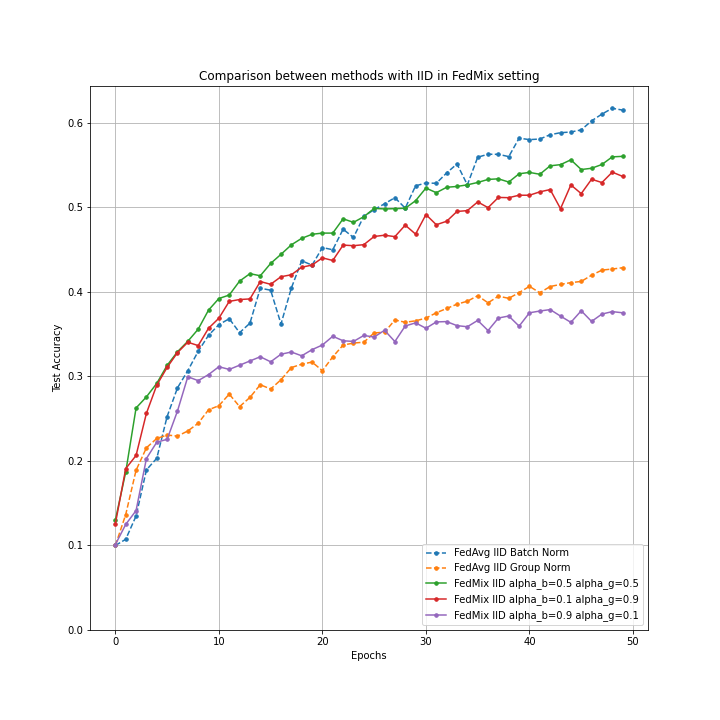
\includegraphics[width=\columnwidth]{Images/Comparison between methods with IID in FedMix setting.png}
    \caption{Comparison between methods with IID in FedMix setting}
    \label{fig:appendix1}
\end{figure}
\begin{figure}[htb]
    \centering
    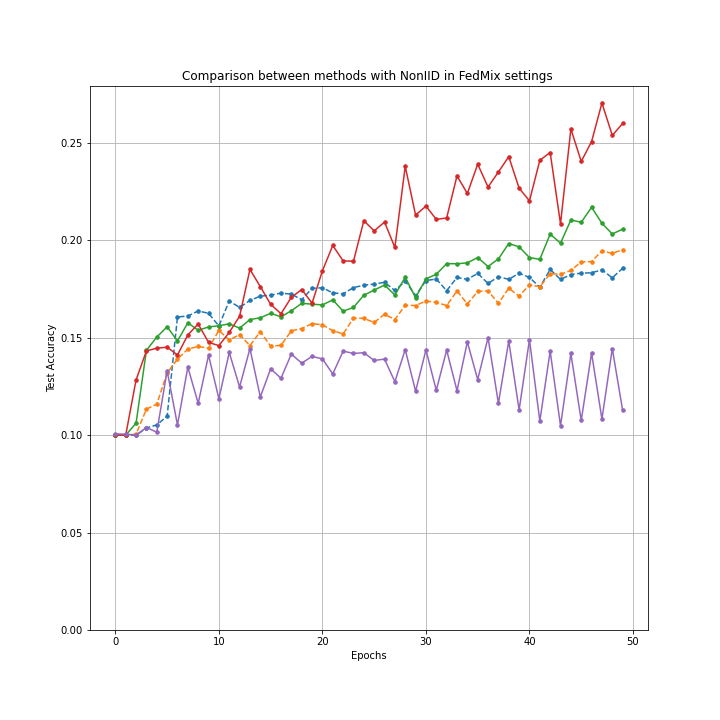
\includegraphics[width=\columnwidth]{Images/Comparison between methods with NonIID in FedMix settings.png}
    \caption{Comparison between methods with NonIID in FedMix settings}
    \label{fig:appendix2}
\end{figure}
\begin{figure}[htb]
    \centering
    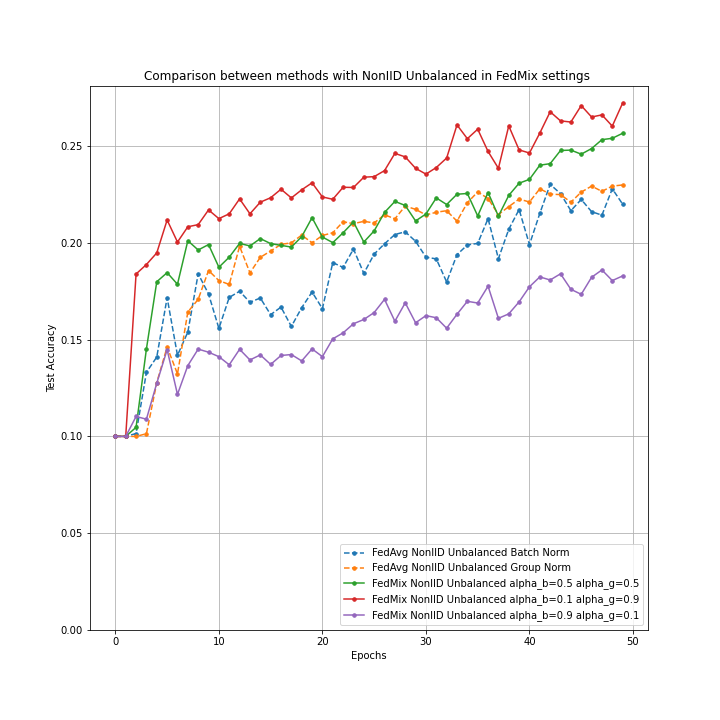
\includegraphics[width=\columnwidth]{Images/Comparison between methods with NonIID Unbalanced in FedMix settings.png}
    \caption{Comparison between methods with NonIID Unbalanced in FedMix settings}
    \label{fig:appendix3}
\end{figure}
\begin{figure}[htb]
    \centering
    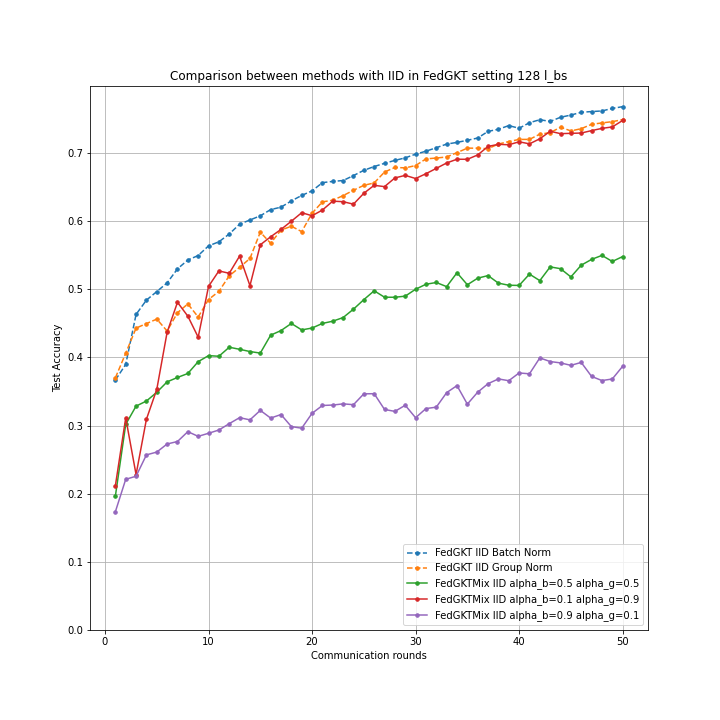
\includegraphics[width=\columnwidth]{Images/Comparison between methods with IID in FedGKT setting 128 l_bs.png}
    \caption{Comparison between methods with IID in FedGKT setting 128 local bs}
    \label{fig:appendix4}
\end{figure}
\begin{figure}[htb]
    \centering
    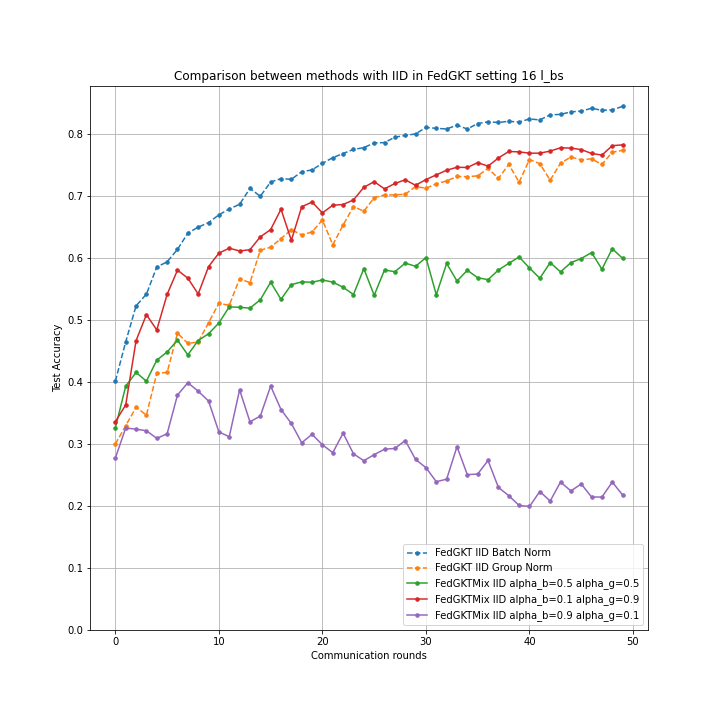
\includegraphics[width=\columnwidth]{Images/Comparison between methods with IID in FedGKT setting 16 l_bs.png}
    \caption{Comparison between methods with IID in FedGKT setting 16 local bs}
    \label{fig:appendix5}
\end{figure}
\begin{figure}[htb]
    \centering
    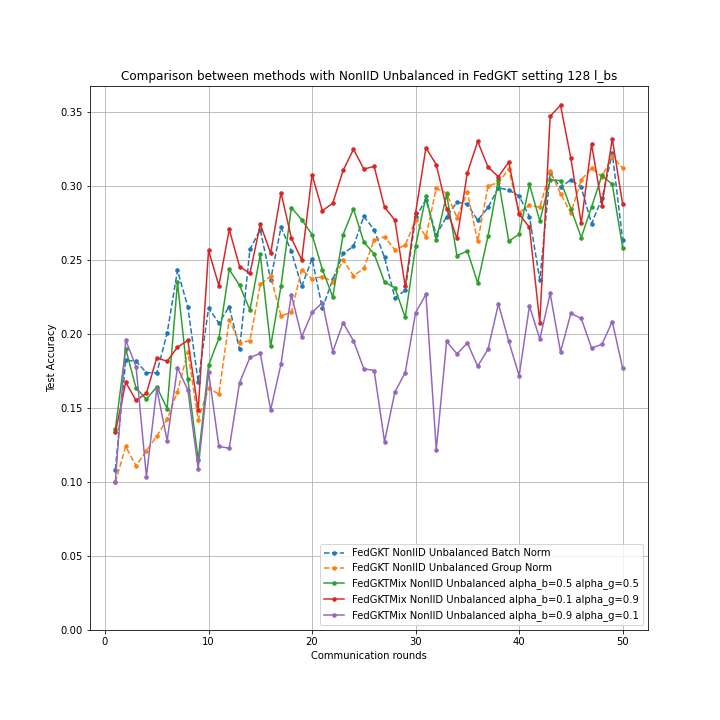
\includegraphics[width=\columnwidth]{Images/Comparison between methods with NonIID Unbalanced in FedGKT setting 128 l_bs.png}
    \caption{Comparison between methods with NonIID Unbalanced in FedGKT setting 128 local bs}
    \label{fig:appendix6}
\end{figure}
\begin{figure}[htb]
    \centering
    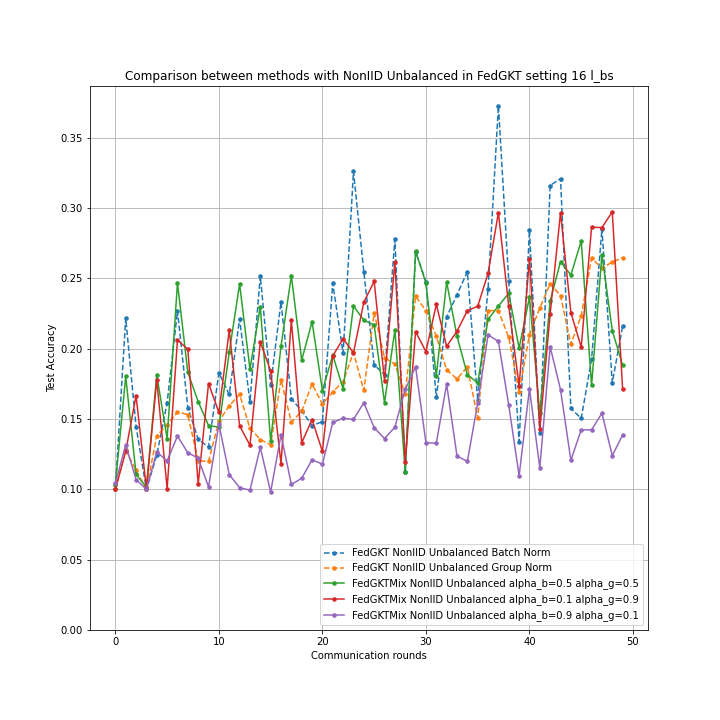
\includegraphics[width=\columnwidth]{Images/Comparison between methods with NonIID Unbalanced in FedGKT setting 16 l_bs.png}
    \caption{Comparison between methods with NonIID Unbalanced in FedGKT setting 16 local bs}
    \label{fig:appendix7}
\end{figure}
\begin{figure}[htb]
    \centering
    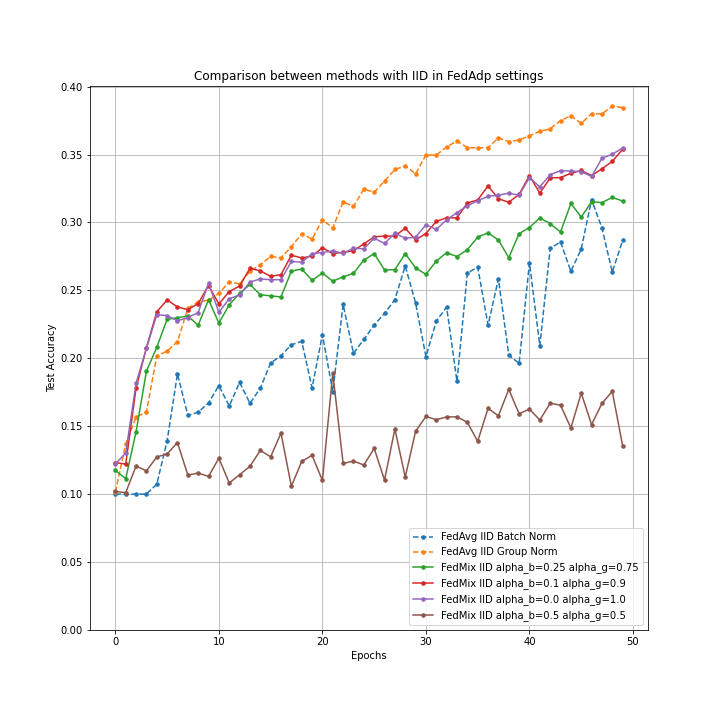
\includegraphics[width=\columnwidth]{Images/Comparison between methods with IID in FedAdp settings.png}
    \caption{Comparison between methods with IID in FedAdp settings}
    \label{fig:appendix8}
\end{figure}
\begin{figure}[htb]
    \centering
    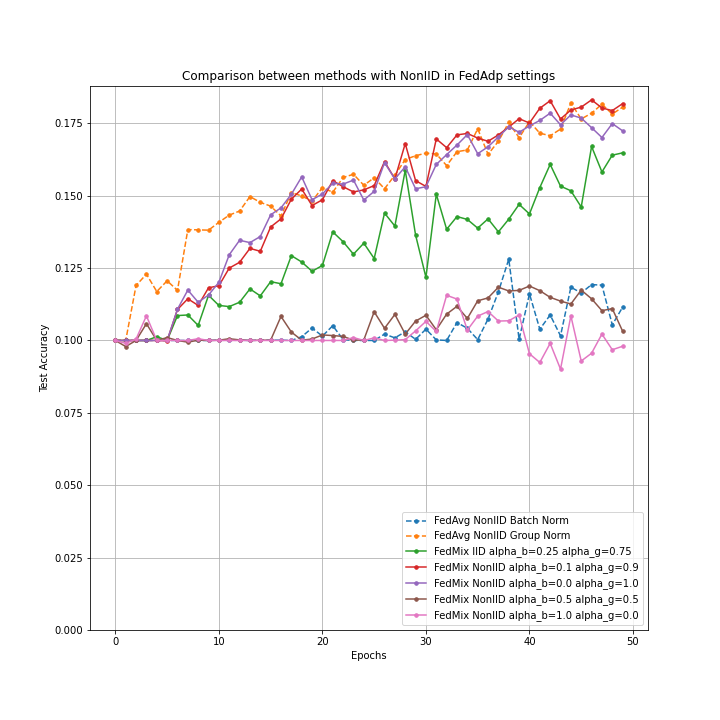
\includegraphics[width=\columnwidth]{Images/Comparison between methods with NonIID in FedAdp settings.png}
    \caption{Comparison between methods with NonIID in FedAdp settings}
    \label{fig:appendix9}
\end{figure}
\begin{figure}[htb]
    \centering
    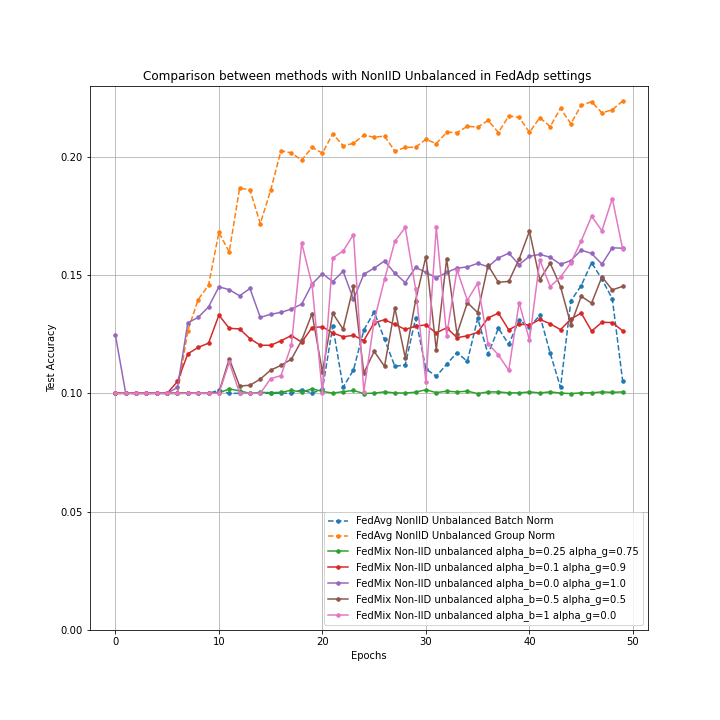
\includegraphics[width=\columnwidth]{Images/Comparison between methods with NonIID Unbalanced in FedAdp settings.png}
    \caption{Comparison between methods with NonIID Unbalanced in FedAdp settings}
    \label{fig:appendix10}
\end{figure}



\begin{table}[htb]
\caption{Comparison between parameters in centralized method}
\begin{tabular}{|p{0.15\columnwidth}|p{0.15\columnwidth}|p{0.15\columnwidth}|p{0.15\columnwidth}|p{0.15\columnwidth}|}
\hline
{\textbf{\begin{tabular}[c]{@{}c@{}c@{}}\centerline{Norm}\end{tabular}}} 
& {\textbf{\begin{tabular}[c]{@{}c@{}c@{}}Learning \\ rate\end{tabular}}}
& {\textbf{\begin{tabular}[c]{@{}c@{}}\centerline{Momentum} \\\end{tabular}}}
& {\textbf{\begin{tabular}[c]{@{}c@{}c@{}}\centerline{Optimizer}\end{tabular}}}
& {\textbf{\begin{tabular}[c]{@{}c@{}c@{}}Test \\ Accuracy \\(\%)\end{tabular}}}\\ \hline

\rule[-4mm]{0mm}{1cm} {BN} & \centerline{0.001} & \centerline{0.5} & \centerline{SGD} & \centerline{66.0}\\\hline
\rule[-4mm]{0mm}{1cm} {BN} & \centerline{0.001} & \centerline{0.9} & \centerline{SGD} & \centerline{76.0}\\\hline
\rule[-4mm]{0mm}{1cm} {BN} & \centerline{0.1} & \centerline{0.5} & \centerline{SGD} & \centerline{81.0}\\\hline
\rule[-4mm]{0mm}{1cm} {BN} & \centerline{0.1} & \centerline{0.9} & \centerline{SGD} & \centerline{85.0}\\\hline
\rule[-4mm]{0mm}{1cm} {BN} & \centerline{0.001} & \centerline{0.5} & \centerline{Adam} & \centerline{87.0}\\\hline
\rule[-4mm]{0mm}{1cm} {BN} & \centerline{0.001} & \centerline{0.9} & \centerline{Adam} & \centerline{87.0}\\\hline
\rule[-4mm]{0mm}{1cm} {BN} & \centerline{0.1} & \centerline{0.5} & \centerline{Adam} & \centerline{85.0}\\\hline
\rule[-4mm]{0mm}{1cm} {BN} & \centerline{0.1} & \centerline{0.9} & \centerline{Adam} & \centerline{85.0}\\\hline
\rule[-4mm]{0mm}{1cm} {GN} & \centerline{0.001} & \centerline{0.5} & \centerline{SGD} & \centerline{73.0}\\\hline
\rule[-4mm]{0mm}{1cm} {GN} & \centerline{0.001} & \centerline{0.9} & \centerline{SGD} & \centerline{80.0}\\\hline
\rule[-4mm]{0mm}{1cm} {GN} & \centerline{0.1} & \centerline{0.5} & \centerline{SGD} & \centerline{81.0}\\\hline
\rule[-4mm]{0mm}{1cm} {GN} & \centerline{0.1} & \centerline{0.9} & \centerline{SGD} & \centerline{83.0}\\\hline
\rule[-4mm]{0mm}{1cm} {GN} & \centerline{0.001} & \centerline{0.5} & \centerline{Adam} & \centerline{81.0}\\\hline
\rule[-4mm]{0mm}{1cm} {GN} & \centerline{0.001} & \centerline{0.9} & \centerline{Adam} & \centerline{81.0}\\\hline
\rule[-4mm]{0mm}{1cm} {GN} & \centerline{0.1} & \centerline{0.5} & \centerline{Adam} & \centerline{77.0}\\\hline
\rule[-4mm]{0mm}{1cm} {GN} & \centerline{0.1} & \centerline{0.9} & \centerline{Adam} & \centerline{77.0}\\\hline
\end{tabular}
\label{tab:1}
\end{table}




\vspace{12pt}
\end{document}
